\documentclass{sig-alternate-05-2015}

\usepackage{xcolor}

\newcommand{\note}{\color{red}$*$}

\begin{document}

\tolerance=10000 

\title{Synthesis-Aided Compiler for Manycore Computation}
\subtitle{Midterm Report}

\numberofauthors{1} 
\author{
\alignauthor
Alexa VanHattum\\
       \affaddr{Cornell University: CS 6410: Advanced Systems}\\
       \email{avh@cs.cornell.edu}
}
\date{1 November 2018}

\maketitle

{\note Idea for this draft: have an Introduction, Related Work, and Design in fairly good shape for the final report (which should be about 10 pages). Plus, an implementation and evaluation plan that ``describe how you plan to implement the system (esp. the details of how it situates in the OS environment) and what experiments you will run on your final system.'' }
\begin{abstract}

Novel, programmable computer architectures offer developers orders-of-magnitude performance improvements over traditional CPUs or GPUs for certain classes of computation, such as dense matrix computation. However, compiling programs to run on such hardware ``accelerators'' is an arduous task. An efficient, optimized compiler for a new architecture may take multiple engineer-years of work to build, much of which is specific only to that target accelerator. We are creating a compiler for a re-configurable, ``manycore'' architecture that partitions and maps computation across a grid of distinct, simple processor cores. Our compiler will leverage program synthesis, a core programming languages technology used to automate the construction of programs, to spatially map computation without relying on traditional hand-written optimizations. This work will ultimately allow developers to write programs for new, efficient hardware accelerators without learning to write dense low-level code themselves or waiting for an optimized compiler to be developed via traditional mechanisms. In addition, we expect such synthesis-aided compiler technology to be more flexible for compiling to distinct but related architectures in the future.

{\note TODO: add in simulated experimental results once I have them} 

\end{abstract}


%
% The code below should be generated by the tool at
% http://dl.acm.org/ccs.cfm
% Please copy and paste the code instead of the example below. 
%
\begin{CCSXML}
<ccs2012>
<concept>
<concept_id>10011007.10011006.10011041.10011043</concept_id>
<concept_desc>Software and its engineering~Retargetable compilers</concept_desc>
<concept_significance>500</concept_significance>
</concept>
<concept>
<concept_id>10011007.10011006.10011008.10011024.10011034</concept_id>
<concept_desc>Software and its engineering~Concurrent programming structures</concept_desc>
<concept_significance>500</concept_significance>
</concept>
</ccs2012>
\end{CCSXML}
\ccsdesc[500]{Software and its engineering~Retargetable compilers}
\ccsdesc[500]{Software and its engineering~Concurrent programming structures}

%
% End generated code
%

%
%  Use this command to print the description
%
\printccsdesc

\keywords{Program Synthesis, Compilers, Reconfigurable Architecture, Spacial Architecture}

\section{Introduction}
To create the most performant applications, software developers are increasingly exploring the use of programmable hardware accelerators. One promising style of accelerator (especially popular in embedded computing) combines many small, simple, independent processor cores. While such ``manycore'' accelerators can offer huge performance gains, their use necessitates unfamiliar and low-level programming models that may be hard for developers to navigate. For example, new hardware may be designed by computer architects to support only a language at about the same abstraction level as an assembly language, but with additional unfamiliar syntax. Specialized compilers from high-level languages offer more programmability to application developers. However, because the design and manufacturing of specialized accelerators may be one-off, compiler engineers then find themselves in a race against time to optimize for an unfamiliar architecture that may be surpassed in a few short years. Further, it may take multiple engineer-years to develop an optimized compiler for a new architecture, leaving application developers without many options in the meantime beyond writing low-level code themselves.

\begin{figure}
\centering
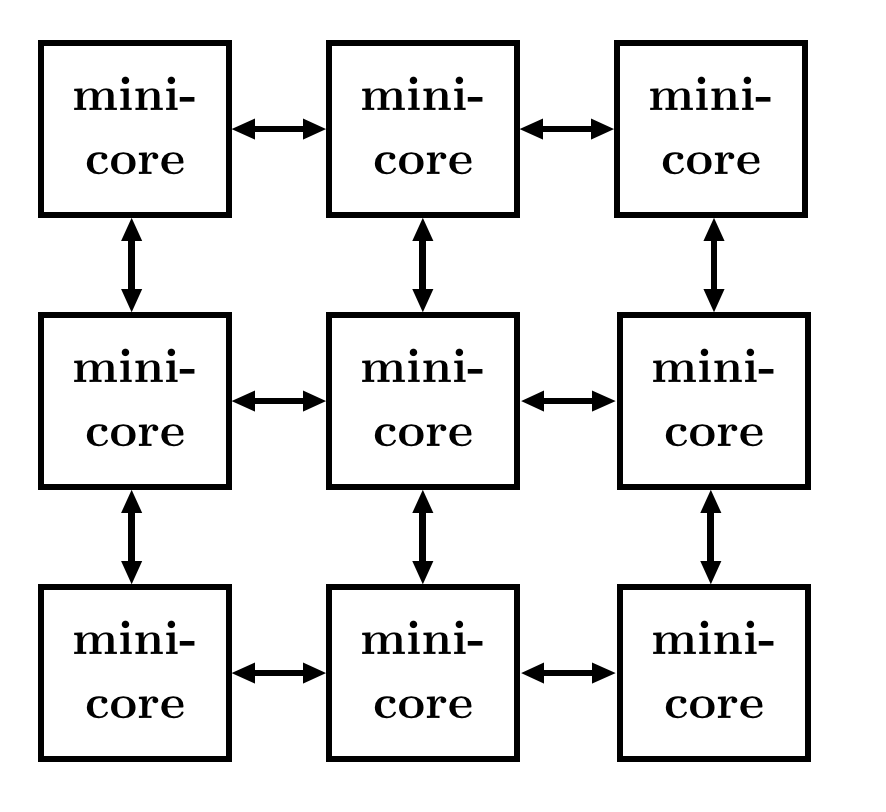
\includegraphics[width=1.7in]{core-grid.png}
\caption{A $3 \times 3$ grid of mini-cores processors. As shown, each core can only communicate directly with 4 (or fewer) immediately adjacent cores. {\note Make this graphic more interesting? Show zoomed in detail of a core and/or routing between cores?}}
\end{figure}

Compiling programs to run efficiently on a manycore architecture poses numerous challenges. First, unlike when compiling for a traditional CPU architecture, there is no underlying operating system that handles the scheduling of processes and threads across the several cores. Rather, it is the responsibility of either the programmer (if they are writing low-level code directly) or the compiler to partition and schedule the computation across the multitude of cores. Second, in addition to partitioning the program per-core, this programming model also requires that some or all data communication be explicitly sent between neighboring cores (see Figure 1). If data needs to move between cores that are not adjacent, it must be sent pair-wise along a route of connected cores, causing communication forwarding to have to contend with other partitions of the program running on those intermediate cores. In addition, some architectures aim to offer even more degrees of freedom by allowing the software layer to re-configure the hardware. For example, the software stack may be able to dictate that one core is allowed to ``shutdown'' a neighbor in order to pool the resources of the two cores together for a single sub-computation. 

Program synthesis, or the automated construction of programs from a high-level specification, offers the promise of programmability without sacrificing lower-level performance and optimizations. For example, program synthesis has been shown to be effective at aiding the development of a compiler for a specific super-low-power manycore architecture, the GreenArrays GA114~\cite{chlorophyll}. The problem of compiling from a higher-level language to the instruction set for the GreenArrays spatial, manycore architecture is expressed as a series of constraints that can be solved with an off-the-shelf SMT, or Satisfiability Modulo Theory, solver. SMT solvers work by encoding complex systems of constraints within a combination of boolean algebra and a series of ``theories'', such as the Theory of Linear Arithmetic for equality constraints over integers. Solvers then use efficient search algorithms to find an assignment of variables such that the given formula holds true. For the case of program synthesis, the challenge is to encode the construction of programs into a system of constraints that can be understood by the SMT solver. {\note Do I need more explanation of SMT here? Could add a separate background subsection for it.}

I am working with Professor Adrian Sampson to extend this line of research by developing tooling to efficiently map higher-level application programs across a re-configurable manycore architecture. In particular, I will develop a model of the spatial layout of a given architecture along with an estimated cost model for the efficiency of communication across cores. Figure 1 shows an example manycore communication layout. I will then leverage program synthesis to find a partitioning of the high-level program across the cores that minimizes the cost function. I will ultimately compile code to a basic instruction set based on RISC-V, an open and extensible Instruction Set Architecture (ISA)~\cite{risc-v}. We can then use hardware simulators to evaluate how the performance of the synthesis-aided compiler compares to the application running on a single core. This line of work aims to give developers the ability to write performant manycore applications at a higher level, without waiting for specialized compilers to be created or learning to hand-write optimized low-level code themselves. In addition, there have only been a handful of existing systems that have used program synthesis or SMT solvers to aid in compilation \cite{chlorophyll, alive, optgen, souper, future}. We hope that ultimately, the insights we gain from this project can be leveraged in creating efficient and correct compilers for applications beyond just those targeting manycore architectures. 

\section{Related Work}

\subsection{Compilers for Parallelization}
There has been significant work on the general problem of compiling domain-specific, higher-level applications to optimize for particular architectures. For example, for deep learning applications, the TVM compiler can optimize for multiple back-ends, including GPUs and FPGA-based accelerators~\cite{tvm}. However, TVM does not yet support manycore architectures, and it is targeted for machine-learning-specific languages. In general, parallelization of higher-level applications has focused on commodity hardware including CPUs, GPUs, and increasingly FPGAs, but has not addressed the potential of compiling to specialized, reconfigurable manycore architectures. 
{\note I definitely need to add more here if I want to cite TVM: TensorFlow? Non-ML-based automated parrallelization?}

\subsection{Compilers for Manycore Architectures}
Most of the existing compilers for manycore architectures are based on heuristics, rather than program synthesis or constraint solving as a general approach. For example, the RAW compiler (RAWCC) compiles general-purpose sequential programs in C or Fortran to a distributed spacial architecture~\cite{raw}. Because the problem of optimally scheduling computation in space and time is typically NP-complete {\note citation?}, RAWCC uses a set of greedy heuristics to create approximate solutions. In particular, they decompose the compilation problem into traditional compiler optimizations, clustering of instructions, merging of instruction clusters until they fit within the number of compute units, then globally partitioning data. However, the Raw compiler only targets a specific Raw architecture, so each optimization came at the cost of being specifically designed by a compiler engineer. {\note Cite heuristic spatial compilers other than Raw?}

\subsection{Constraint-Guided Compilation}
As described by Lopes and Regehr in \emph{Future Directions for Optimizing Compilers}~\cite{future}, there is increasingly interest in using satisfiability modulo theories (SMT, the core technology behind many forms of program synthesis) and other constraint-based solvers to improve compiler speed, correctness, and generated code quality. However, this area of work is still in the early stages. In particular, because SMT solvers and systems for program synthesis must exhaustively enumerate search spaces, their clients must contend with issues of scalability as problem sizes approach realistic system sizes. 

Alive is a domain-specific language (DSL) for writing efficient and correct compiler optimizations for LLVM, a popular language-agnostic compiler toolchain~\cite{alive}. Alive uses an SMT solver to automatically prove an optimization correct (or, conversely, to provide a counterexample demonstrating its incorrectness). Alive was effective in finding eight previously unknown bugs in an existing LLVM optimization. Optgen is another SMT-based compiler tool that was used to find previously unknown optimizations for GCC, LLVM, and ICC~\cite{optgen}. Souper is a similar, but less mature, super-optimizing compiler that uses SMT-solving and also integrates with LLVM~\cite{souper}. {\note ``less mature'' in that the papers seems to only give its weaknesses compared to other systems, and it hasn't been published outside of arxiv yet (?). Better ways to say this?} Each of these systems focus on optimizing components of existing compilers that mostly target commodity CPUs, rather than leveraging an SMT solver for spatial partitioning for more specialized architectures.

There has also been some previous work using Integer Linear Programming (ILP) constraint solvers to schedule computation across spatial architectures~\cite{ilp}. However, much of the previous focus in that area has been on mapping data flow graphs onto fixed, specific spatial architectures. They are not as flexible, and do not consider architectures that may support reconfiguration. For example, we imagine supporting an manycore architecture where some adjacent cores may pool resources for particularly large pieces of computation. 

Chlorophyll is a synthesis-aided compiler from a custom C-like domain-specific language (DSL) to a particular super-low-power manycore architecture, the GreenArrays GA114~\cite{chlorophyll}. Chlorophyll addresses scalability challenges by dividing the compilation into smaller sub-problems: (1) partitioning computation across cores, (2) layout of logical computation partitions onto physical cores, (3) code separation to divide source code and insert communication code, and (4) code generation to ``super-optimize'' instructions. We plan to leverage the insight from Chlorophyll to separate compiler concerns into phases to enable tractable synthesis that can reasonably scale. However, unlike Chlorophyll, our system aims to support re-configurable architecture rather than than only one specific manycore architecture like the GreenArrays GA114. In addition, the Chlorophyll DSL imposes restrictions particular to the GA114's cores' limitations, including disallowing recursion and arbitrary array indexing. Because the cores in the architectures we imagine targeting will not be as restricted, we would like to be able to support a more flexible high-level programming model (although almost certainly not within the scope of this semester). 

\begin{figure}
    \centering
    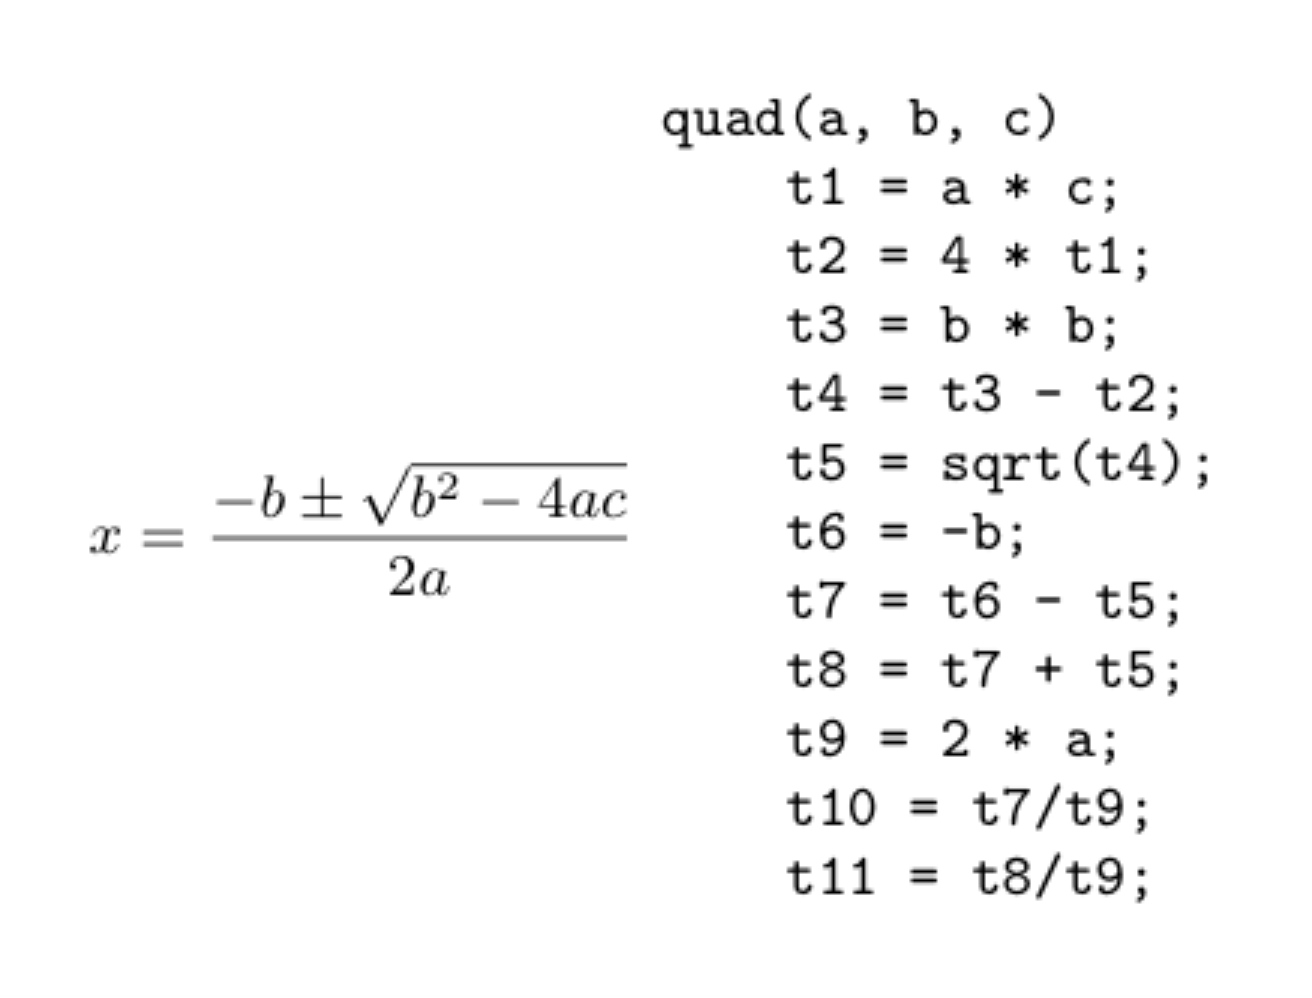
\includegraphics[width=3in]{quadratic.png}
    % $$x=\frac{-b\pm\sqrt{b^2-4ac}}{2a}$$
    % \begin{verbatim}
    % quad(a, b, c)
    %     t1 = a * c;
    %     t2 = 4 * t1;
    %     t3 = b * b;
    %     t4 = t3 - t2;
    %     t5 = sqrt(t4); 
    %     t6 = -b;
    %     t7 = t6 - t5;
    %     t8 = t7 + t5;
    %     t9 = 2 * a;
    %     t10 = t7/t9;
    %     t11 = t8/t9;
    % \end{verbatim}
    \caption{The quadratic formula (left) expressed as a computation in Static Single-Assignment (SSA) form (right). The roots of the quadratic equation specified by variables $a$, $b$, and $c$ are computed to be the final variables of $t10$ and $t11$.}
    \label{fig:my_label}
\end{figure}

\section{Design}
One key insight from previous work in using program synthesis for compilation is that in order to scale, compiling must be broken up into several sub-problems. Our system design includes components for (1) compiling from a higher-level language to Static Single-Assignment (SSA) intermediate form, (2) compiling the SSA form into a Data Flow Graph (DFG), (3) mapping that data flow graph over the manycore architecture model using an SMT solver, and (4) generating RISC-V instructions per processor core. {\note This entire section is pretty seat-of-my-pants and needs a lot more detail once I get more things working}

\subsection{Compiling the Higher-Level Language}
While we would like to eventually support an expressive and flexible high-level language at a similar abstraction level (if significantly less mature) than something like Python, within the scope of one semester this is not feasible. Rather, I am focusing on starting with a very small, very simple imperative language that can be built upon incrementally. The initial language will likely only support simple data types such a integers, floats and booleans and exclude stucts or tuples. I will create a lexer, parser, and compiler for this language using OCaml, a popular functional programming language that offers convenient libraries for language building. 

\subsection{Static Single-Assignment Form}
Static-Single Assignment (SSA) form is a imperative programming model that requires that every variable is assigned to exactly once, and that every variable is defined before it can be used. This is an especially useful representation for a compiler, because SSA form has a direct translation into a Data Flow Graph (DFG) that models dependencies between operations that process data. Data flow graphs are used in many traditional compiler optimizations such as reaching definition analysis, where writes to variables that are overwritten before the variable is read can be safely removed from the computation. Figures 2 and 3 illustrate a static single-assignment form expression and a data flow graph for the quadratic formula (the equation for finding the roots of a quadratic expression). As you can see, the data flow graph makes data dependencies between different operations explicit. 
\begin{figure}
\centering
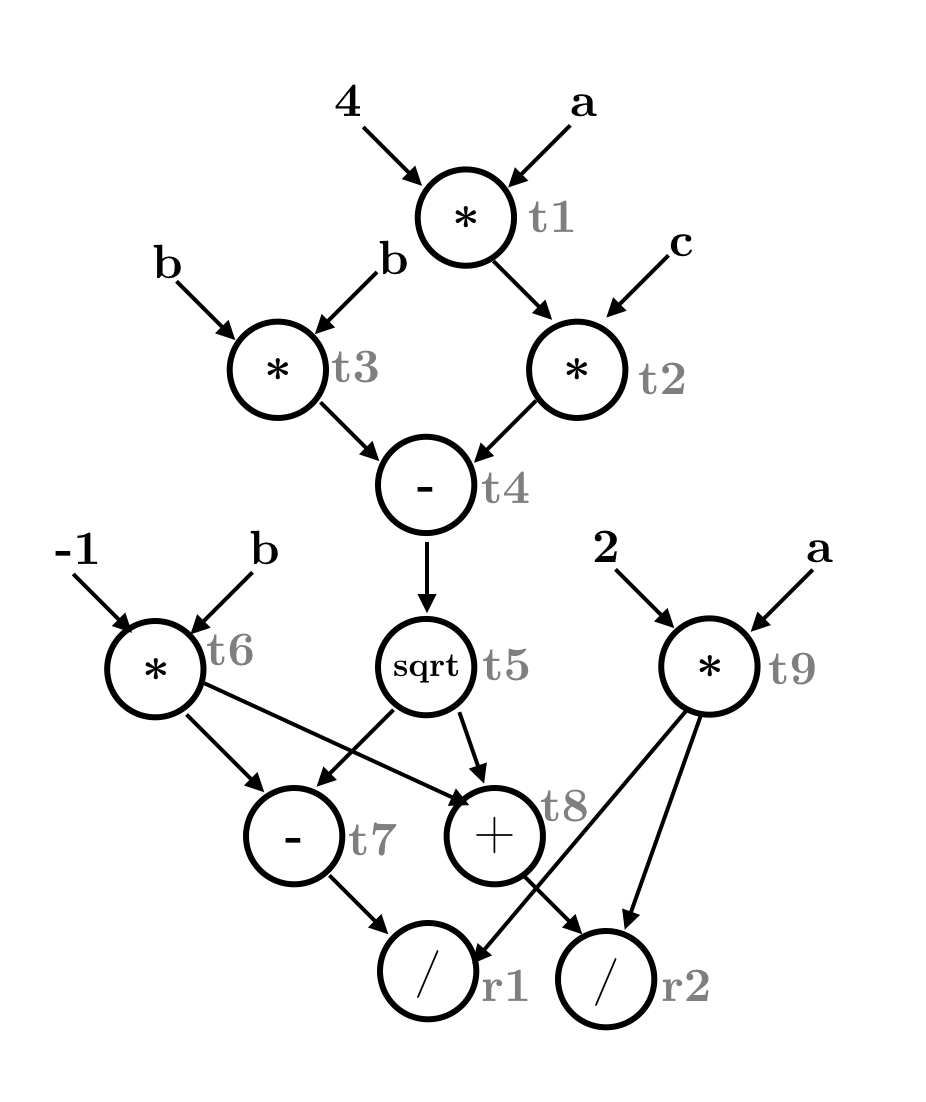
\includegraphics[width=3in]{data-flow.png}
\caption{The data flow graph for the quadratic formula computation shown in Figure 2. Each node is labeled with the variable used in the SSA form expression, as well as the operation used. {\note This is wrong, oops}}
\end{figure}
For this project, I will use a data flow graph representation in order to analyze how to partition computation across cores such that data dependencies are met. In the quadratic formula example, it would be possible for the multiplication operation at \texttt{t1} and the multiplication operation at \texttt{t3} to occur simultaneously on different cores, since they do not have any data dependencies. However, the subtraction operation at \texttt{t4} cannot be mapped to perform simultaneously with the previous operations, since it is dependent on their output. 

The compiler passes from the high-level language to SSA form and from SSA form to a data flow graph will both be straightforward, syntax-driven program transformations. 

\subsection{Mapping to Manycore}
Once the program representation is in a data flow graph, mapping it to the manycore architecture involves solving a series of constraints on space, time, and communication costs. For constraint solving, we are using Microsoft Research's Z3 SMT solver \cite{z3}. {\note this and the next paragraph especially need more detail}

First, we will generate a series of constraints that represent the manycore architecture using the SMT Theory of Uninterpreted Functions, which models first-order predicate logic. We will then use Z3 to quantify over all programs that could be generated from the starting conditions that satisfy the modeled constraints and are semantically equivalent to the data flow graph. Each potential program will be modeled such that satisfying instances include an estimated cost for that program. Once we have a candidate program, we will incrementally ask Z3 to find another satisfying instance with the additional constraint that the newer program has a \emph{lower} cost than the most efficient program we have found thus far. We will then repeat this process until no satisfying instances are found. Z3 is able to save internal states between search executions, which we will leverage in this strategy of incrementally increasing the difficulty of the cost constraint.

It may be the case that the strategy outlined about does not scale to a reasonably sized manycore grid. In that case, we may need to further divide the problem. For example, we may use a distinct set of constraints to model diving the computation per-core, and then a new set of constraints for communicating across cores. 

\subsection{Generating Instructions}
Finally, once we have a program that efficiently maps the data flow graph onto the model of the spacial manycore grid, we need to partition the program into per-core sub-programs in a low-level language. 

We have chosen to base our target low-level language on RISC-V because it is an open and extensible instruction set architecture. The RISC-V distribution also includes a cycle-level simulator, which is described in more detail in the evaluation plan. 

In particular, RISC-V includes a small base of core instructions and numerous optional extensions. New functionality can be added via custom extensions. We plan to base our target language on the RISC-V base plus a small extension to model communication between cores. The compiler pass from the data flow graph and core model to this instruction set will again be heuristic-based program transformation. This transformation will include both mapping the components of the data flow graph into instructions, and adding communication instructions as needed to translate information between cores. {\note unclear whether I should instead describe roughly basing the target ISA on RISC-V without actually using the base and an extension, and specify that the actual alignment w/ a real instruction set will come much later}

\section{Implementation Plan}
As a first step, I have created a lexer, parser, and interpreter for a very simple language already consistent with Static Single-Assignment (SSA) form in OCaml. In this language, the only supported type is 64-bit floating-point numbers. Boolean computations are represented with floats, as they are implicitly in many C-based languages. I currently have a compiler pass that enforces the SSA form, and have begun the next pass to transform the SSA form abstract syntax tree into a data flow graph.

In parallel, I am using Z3's Python bindings to construct a model of the SMT constraints for the many-core architecture. Currently, the model makes many simplifying assumptions about the manycore architecture (for example, that each core can read program input from any location). My next step is to finish the compiler transformation from SSA form to a data flow graph. Once that is complete, I will begin integrating the data flow graph representation with my Z3 model of the architecture constraints.

Once I have this minimal functional synthesis-aided compiler that can map the data flow graph onto the idealized model of the manycore architecture, I will begin the last pass of the compiler, from the partitioned mapping to the RISC-V instruction set. 

Finally, I will implement the front-end of the compiler, from the higher-level language to the SSA form I have been working with thus far. I've chosen to leave that component for later in the course of this project because it is almost entirely language design, and less directly relevant to building efficient systems. 

In addition, I have the following area of investigation as a stretch-goal for the semester. Ultimately, we would like to allow components of the spatial architecture layout to be symbolic; that is, also leverage program synthesis to inform decisions about how the hardware can be optimally (re-)configured. This involves leaving some components of the Z3 model, such as the constraints that restrict maximum computation size per core, as symbolic variables that can be modified later in the analysis. 

\section{Evaluation Plan}
Another student in Professor Adrian Sampson's Computer Architecture and Programming Abstractions (CAPRA) group is in the process of developing a first-order, cycle-level simulator of the re-configurable manycore architecture. This simulator current supports running arbitrary functions in C++ on each simulator core, as well as communication between the cores. The simulator also allows you to specify per function the estimated cost of that computation. I plan to evaluate the performance of the RISC-V instructions generated by the new synthesis-aided compiler by running them on this simulator. To do so, I will need to write an interpreter in C++ for the RISC-V instruction set I plan to utilize. My existing interpreter for the SSA (single-static assignment) language should be able to inform my implementation of the C++ interpreter. In addition, I will include the estimates for the cycle cost per instruction, such that the interpreter can estimate the total cost as well as evaluating the computation. {\note will I actually be able to/need to do this? Or should I just use the cost output by my model directly? I like the idea of comparing across simulators if I have time.}

For comparison, I will evaluate semantically equivalent computations in the pure RISC-V instruction set by running them on Spike, an open-source RISC-V Instruction Set Architecture (ISA) simulator \cite{risc-v}. I can use the number of cycles output between the two simulators as a proxy for the performance of the compiled code. In addition, Spike allows you to configure the number of simulated cores. Thus, I can evaluate how the performance improvements gained from compiling for a manycore architecture compares relative to gains from adding additional cores within the context of a more traditional operating system and architecture. {\note this may actually be too tricky?} Finally, I have a stretch-goal for the semester to evaluate how the performance of programs from the synthesis-aided compiler compares to that of equivalent programs: (1) hand-crafted with lower-level languages targeting the manycore hardware, and (2) from more traditional heuristic-based compiler algorithms that target spatial architectures, such as those used by Raw~\cite{raw}.

This strategy of comparing results across two distinct simulators is not an extremely accurate evaluation. In particular, the simulators may make different, influential assumptions about hardware behavior and the associated cycle-level statistics. However, such a simulator comparison is necessary because the targeted manycore architecture does not physically exist yet. In addition, comparing results across simulations will allow us to further explore the design space and thus use the compiler development to help inform the decisions made in designing the hardware.
\bibliographystyle{abbrv}
\bibliography{refs} 

\end{document}
